\documentclass[11pt,a4paper]{article}
\usepackage[T1]{fontenc}
\usepackage[utf8]{inputenc}
\usepackage{lmodern}
\usepackage{microtype}
\usepackage[margin=2.5cm]{geometry}
\usepackage{amsmath,amssymb,mathtools}
\usepackage{graphicx}
\usepackage{booktabs}
\usepackage{array}
\usepackage{caption}
\usepackage{subcaption}
\usepackage{float}
\usepackage{xcolor}
\usepackage{fancyhdr}
\usepackage{enumitem}
\usepackage[most]{tcolorbox}
\usepackage{tikz}
\usetikzlibrary{arrows.meta,positioning,calc,shapes.geometric,decorations.pathmorphing,fit}
\usepackage[colorlinks=true,linkcolor=navy,urlcolor=navy,citecolor=navy]{hyperref}

\definecolor{navy}{HTML}{1F4E79}
\definecolor{brick}{HTML}{C0504D}
\definecolor{leaf}{HTML}{4F8F3A}
\definecolor{sand}{HTML}{F4F1EA}

\graphicspath{{figures/}{../img/}}
\captionsetup{font=small,labelfont=bf}
\setlength{\parskip}{0.45em}
\setlength{\parindent}{0pt}
\setlist{itemsep=0.15em,topsep=0.3em}

\pagestyle{fancy}
\fancyhf{}
\fancyhead[L]{\small\textit{helisim: maths and physics guide}}
\fancyhead[R]{\small Ruben Colomina}
\fancyfoot[C]{\small\thepage}
\setlength{\headheight}{14pt}

\newcommand{\code}[1]{\texttt{#1}}
\newcommand{\un}[1]{\,\mathrm{#1}}
\newcommand{\dd}{\mathrm{d}}
\newcommand{\wrap}{\operatorname{wrap}}
\newcommand{\sat}{\operatorname{sat}}
\newcommand{\E}{\mathbb{E}}

\newtcolorbox{devnote}[1][Developer note]{enhanced,breakable,colback=sand,colframe=navy,
  boxrule=0.5pt,arc=1.5pt,left=6pt,right=6pt,top=4pt,bottom=4pt,
  fonttitle=\bfseries\small,title={#1}}
\newtcolorbox{codemap}{enhanced,colback=white,colframe=leaf,boxrule=0.5pt,arc=1.5pt,
  left=6pt,right=6pt,top=3pt,bottom=3pt,fontupper=\small}

\title{\textbf{helisim}\\[0.3em]
\Large A Mathematics and Physics Guide for Developers\\[0.4em]
\large The Mark on Target automatic approach to hover:\\ model, guidance laws and turbulence}
\author{Ruben Colomina}
\date{November 2026 \\[0.3em] \small Describes \code{helisim} version 0.1.0}

\begin{document}
\maketitle
\thispagestyle{empty}

\begin{center}
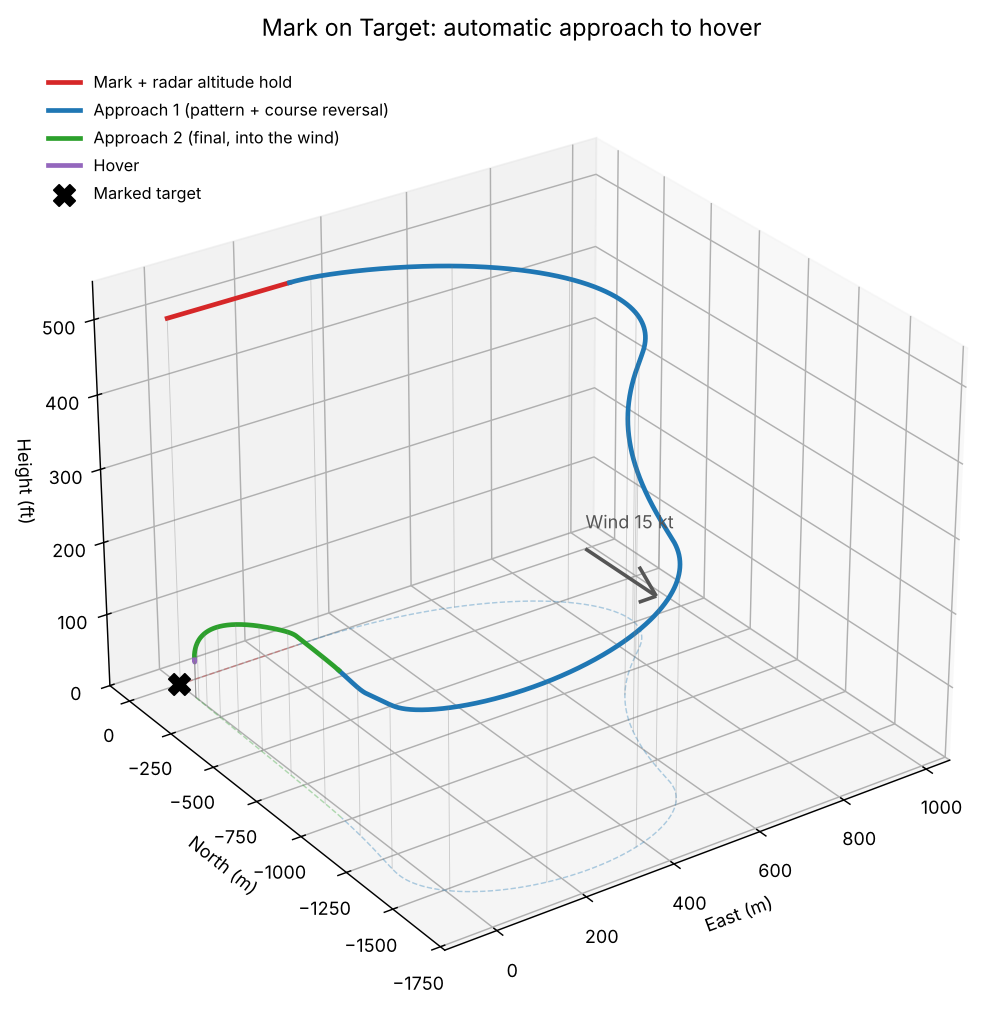
\includegraphics[width=0.78\textwidth]{mot_3d.png}
\end{center}

\begin{abstract}
\noindent This guide explains the mathematics and physics implemented in the
\code{helicopter-afcs-sim} repository, equation by equation, and ties each
equation to the line of code that implements it. It is written for developers
who want to change the simulator and need to know why each formula is there,
what it assumes and what happens when a parameter moves. The annexes collect the
prerequisites (vectors and angles, first- and second-order systems, turn
physics, stochastic processes) so that the main text can be read without other
references.
\end{abstract}

\newpage
\tableofcontents
\newpage

% =====================================================================
\section{Scope and structure of the simulator}

\code{helisim} reproduces the trajectory of a \emph{Mark on Target} (MOT)
automatic approach: the pilot overflies a survivor, presses \emph{Mark}, and
the automatic flight control system (AFCS) flies a pattern that ends in a
hover at $50\un{ft}$, heading into the wind, a short distance downwind of the
marked position.

The simulator is a study tool for \textbf{outer-loop modes}. It does not model
the rotor, the fuselage aerodynamics or the attitude dynamics. Everything the
inner loops of a real AFCS do (stability augmentation, attitude hold) is
replaced by first-order lags and limits. Three blocks interact at every time
step (Figure~\ref{fig:blocks}).

\begin{figure}[H]
\centering
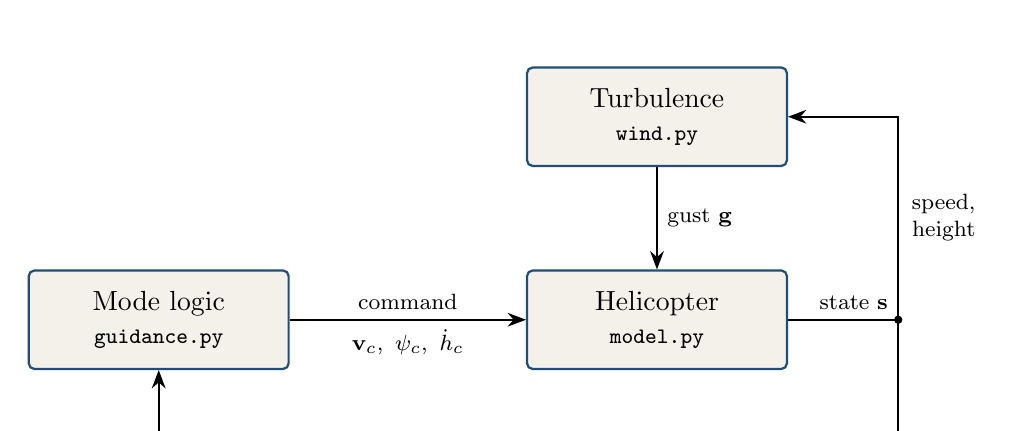
\begin{tikzpicture}[>=Stealth,node distance=1.6cm,
  blk/.style={draw=navy,thick,rounded corners=2pt,minimum width=3.3cm,minimum height=1.25cm,align=center,fill=sand},
  lab/.style={font=\footnotesize,align=center}]
\node[blk] (g) {Mode logic\\\footnotesize\code{guidance.py}};
\node[blk,right=3.0cm of g] (m) {Helicopter\\\footnotesize\code{model.py}};
\node[blk,above=1.3cm of m] (w) {Turbulence\\\footnotesize\code{wind.py}};
\draw[->,thick] (g) -- node[lab,above]{command}node[lab,below]{$\mathbf{v}_c,\ \psi_c,\ \dot h_c$} (m);
\draw[->,thick] (w) -- node[lab,right]{gust $\mathbf{g}$} (m);
\draw[->,thick] (m.east) -- ++(1.4,0) node[lab,above left]{state $\mathbf{s}$} |- ($(g.south)+(0,-0.9)$) -- (g.south);
\draw[->,thick] (m.east)++(1.4,0) |- (w.east);
\node[lab,right] at ($(m.east)+(1.45,1.3)$) {speed,\\height};
\fill (m.east)++(1.4,0) circle (1.5pt);
\end{tikzpicture}
\caption{The simulation loop in \code{sim.py}. Each step: the mode produces a
command from the state, the turbulence model produces a gust, and the
helicopter model advances the state.}
\label{fig:blocks}
\end{figure}

\begin{table}[H]
\centering
\small
\begin{tabular}{@{}lll@{}}
\toprule
File & Content & Section \\
\midrule
\code{params.py} & constants and default parameters & Annex~\ref{app:params} \\
\code{model.py} & point-mass helicopter & \ref{sec:model} \\
\code{wind.py} & Dryden turbulence as a stochastic process & \ref{sec:wind} \\
\code{guidance.py} & pattern geometry, guidance laws, state machine & \ref{sec:geometry}--\ref{sec:guidance} \\
\code{sim.py} & time loop, frame conversion, output & \ref{sec:frames}, \ref{sec:loop} \\
\code{tests/} & properties checked automatically & \ref{sec:tests} \\
\bottomrule
\end{tabular}
\caption{Where each part of the mathematics lives.}
\end{table}

% =====================================================================
\section{Frames, angles and units}\label{sec:frames}

\subsection{The wind-aligned frame}

All the dynamics and guidance are computed in a local frame fixed to the
surface and \emph{aligned with the wind} (Figure~\ref{fig:frame}):
\begin{itemize}
\item the origin is the marked target;
\item $+y$ points \textbf{into the wind}, that is, towards the direction the
wind comes from. The final course is the $+y$ direction;
\item $+x$ points to the right of the final course;
\item $h$ is the height above the surface.
\end{itemize}
Working in this frame makes the pattern independent of the wind direction: the
geometry is always the same and only the conversion to East/North changes.

The heading $\psi$ is stored as a \textbf{mathematical angle}: measured from
$+x$, positive counter-clockwise, in radians. So $\psi=\pi/2$ is ``into the
wind'' and $\psi=-\pi/2$ is ``downwind''. A right turn \emph{decreases} $\psi$.

\begin{figure}[H]
\centering
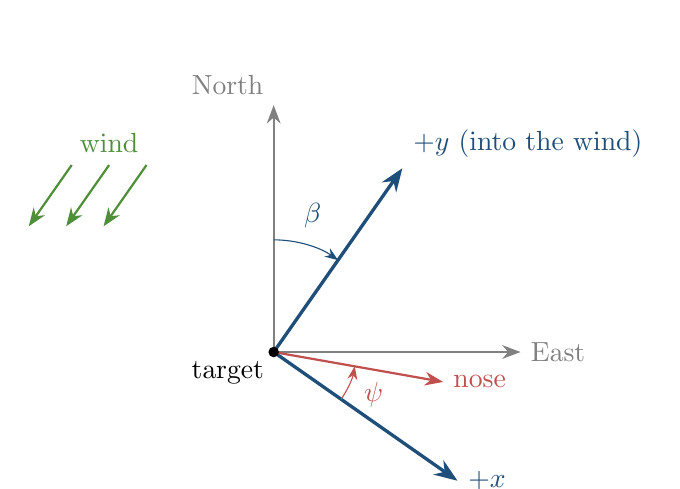
\begin{tikzpicture}[>=Stealth,scale=0.95]
% wind frame rotated by -30 deg relative to north-up page
\draw[->,gray,thick] (0,0) -- (0,3.3) node[above left]{North};
\draw[->,gray,thick] (0,0) -- (3.3,0) node[right]{East};
\begin{scope}[rotate=-35]
  \draw[->,navy,very thick] (0,0) -- (0,3.0) node[above right]{$+y$ (into the wind)};
  \draw[->,navy,very thick] (0,0) -- (3.0,0) node[right]{$+x$};
  \draw[->,brick,thick] (0,0) -- (25:2.3) node[right]{nose};
  \draw[brick,->] (1.1,0) arc (0:25:1.1);
  \node[brick] at (12:1.45) {$\psi$};

\end{scope}
\draw[navy,->] (0,1.5) arc (90:55:1.5);
\node[navy] at (0.52,1.82) {$\beta$};
\fill (0,0) circle (2pt) node[below left]{target};
\foreach \k in {0,0.5,1.0}
  \draw[->,leaf,thick] (-2.7+\k,2.5) -- ++(-0.574,-0.819);
\node[leaf] at (-2.2,2.8) {wind};
\end{tikzpicture}
\caption{Wind-aligned frame. $\beta$ is the meteorological wind direction
(\code{wind\_from\_deg}), a compass bearing; $\psi$ is the heading as a
mathematical angle from $+x$.}
\label{fig:frame}
\end{figure}

\subsection{Conversions to and from compass quantities}

Let $\beta$ be the bearing the wind comes from and $\chi$ a true (compass)
heading, both clockwise from North. The conversions in \code{sim.py} are
\begin{align}
\psi &= \frac{\pi}{2} - (\chi - \beta), &
\chi &= \bigl(\beta + 90^\circ - \psi\bigr) \bmod 360^\circ, \label{eq:hdg}
\end{align}
and the positions are rotated with
\begin{equation}
\begin{pmatrix} E \\ N \end{pmatrix} =
\begin{pmatrix} \cos\beta & \sin\beta \\ -\sin\beta & \cos\beta \end{pmatrix}
\begin{pmatrix} x \\ y \end{pmatrix}. \label{eq:en}
\end{equation}
A quick check: the unit vector $+y$ maps to $(\sin\beta,\cos\beta)$, which is
the unit vector of bearing $\beta$, as required. The matrix is orthogonal with
determinant $+1$, so distances and the handedness of turns are preserved.

\begin{codemap}
\code{sim.py}: \code{\_local\_to\_en} implements \eqref{eq:en}; \code{psi0} and
\code{hdg} in \code{run\_mark\_on\_target} implement \eqref{eq:hdg}.
\end{codemap}

\subsection{Angle wrapping}

Angle differences are always reduced to $[-\pi,\pi)$ with
\begin{equation}
\wrap(a) = \bigl((a+\pi) \bmod 2\pi\bigr) - \pi .
\end{equation}
Every heading error in the code goes through \code{wrap}, so that an error of
$350^\circ$ is treated as $-10^\circ$ and the aircraft turns the short way.

\subsection{Units}

The code mixes SI and aviation units on purpose, to keep the parameters
readable against the public descriptions of the manoeuvre:

\begin{table}[H]
\centering\small
\begin{tabular}{@{}lll@{}}
\toprule
Quantity & Internal unit & Note \\
\midrule
$x$, $y$, distances & m & \\
$v_x$, $v_y$, gusts & m/s & ground velocity \\
$h$ & \textbf{ft} & \\
$\dot h$ (\code{vz}) & \textbf{ft/s} & reported in ft/min \\
$\psi$ & rad & \\
Parameters & kt, ft, ft/min, deg & converted where they are used \\
\bottomrule
\end{tabular}
\caption{Units of the state. Constants: $1\un{kt}=0.514444\un{m/s}$,
$1\un{ft}=0.3048\un{m}$, $g=9.80665\un{m/s^2}$.}
\end{table}

\begin{devnote}
Height in feet and horizontal position in metres is the most likely source of
unit mistakes when extending the code. Any new term that couples the vertical
and horizontal channels (a glide-slope angle, an energy term) needs an explicit
factor \code{FT}.
\end{devnote}

% =====================================================================
\section{The helicopter model}\label{sec:model}

\subsection{State and command}

The state and the command are
\begin{equation}
\mathbf{s} = (x,\ y,\ h,\ \psi,\ v_x,\ v_y,\ \dot h), \qquad
\mathbf{c} = (\mathbf{v}_c,\ \psi_c,\ \dot h_c,\ r_{\lim}),
\end{equation}
where $\mathbf{v}=(v_x,v_y)$ is the \emph{ground} velocity and $r_{\lim}$ is
an optional turn-rate limit that a mode can impose. The model has three
decoupled channels: heading, horizontal velocity and vertical speed.

\subsection{Heading channel}

The heading follows a proportional law with a rate limit:
\begin{equation}
\dot\psi = r = \sat\bigl(k_\psi\,\wrap(\psi_c-\psi),\ \pm r_{\max}\bigr),
\qquad k_\psi = 1.5\un{s^{-1}}. \label{eq:heading}
\end{equation}
For small errors this is a first-order system with time constant
$1/k_\psi\approx0.67\un{s}$. For large errors the aircraft turns at the
constant rate $r_{\max}$, which comes from the physics of a coordinated turn
(Annex~\ref{app:turn}):
\begin{equation}
r_{\max} =
\begin{cases}
\dfrac{g\tan\phi_{\max}}{V} & V \ge 15\un{kt} \quad\text{(banked turn, } \phi_{\max}=25^\circ)\\[1.0em]
15^\circ/\mathrm{s} & V < 15\un{kt} \quad\text{(pedal turn in the hover)}
\end{cases} \label{eq:rmax}
\end{equation}
with $V=\lVert\mathbf{v}\rVert$. At $90\un{kt}$ this gives $5.7^\circ/\mathrm{s}$
and at $60\un{kt}$, $8.5^\circ/\mathrm{s}$. The loop leaves saturation only
when the error is below $r_{\max}/k_\psi$, about $4^\circ$ at $90\un{kt}$, so
during the pattern the heading channel behaves as ``turn at the bank limit,
then settle exponentially''.

\subsection{Horizontal velocity channel}

The inner loops are represented by a first-order lag towards the commanded
ground velocity, with a limit on the magnitude of the acceleration:
\begin{align}
\mathbf{a}_c &= \frac{\mathbf{v}_c-\mathbf{v}}{\tau_v}, &
\mathbf{a} &= \mathbf{a}_c\,\min\!\Bigl(1,\frac{a_{\max}}{\lVert\mathbf{a}_c\rVert}\Bigr)
 + \frac{1}{\tau_g}\begin{pmatrix} g_v \\ -g_u \end{pmatrix}, &
\dot{\mathbf{v}} &= \mathbf{a}, \label{eq:vel}
\end{align}
with $\tau_v=1\un{s}$, $a_{\max}=3\un{m/s^2}$ and $\tau_g=3\un{s}$. The
saturation scales the vector, it does not clip each component, so the
direction of the commanded acceleration is preserved.

The gust $\mathbf{g}=(g_u,g_v,g_w)$ is expressed in wind axes: $g_u$ along the
wind, $g_v$ across it, $g_w$ vertical. A positive along-wind gust pushes the
aircraft downwind, which is $-y$; hence the vector $(g_v,-g_u)$. The gust
acceleration is added \emph{after} the saturation: the disturbance is not
limited by the control authority.

\textbf{Steady response to a gust.} With a constant command and a constant
gust, $\dot{\mathbf v}=0$ in \eqref{eq:vel} gives
\begin{equation}
\mathbf{v}-\mathbf{v}_c = \frac{\tau_v}{\tau_g}\,(g_v,\,-g_u),
\end{equation}
so with the default values one third of a sustained gust appears as a ground
velocity error. The ratio $\tau_v/\tau_g$ is the gust rejection of the inner
loops: reduce $\tau_v$ or increase $\tau_g$ to model a stiffer aircraft.

\subsection{Vertical channel}

\begin{equation}
\ddot h = \frac{\sat(\dot h_c,\pm \dot h_{\max}) - \dot h}{\tau_h}
 + \frac{g_w}{0.3048\,\tau_g},
\qquad \tau_h = 1\un{s},\quad \dot h_{\max}=1000\un{ft/min}. \label{eq:vert}
\end{equation}
The factor $0.3048$ converts the vertical gust from m/s to ft/s. The height is
clamped at the surface, $h\ge0$.

\subsection{Integration}

The equations are advanced with a fixed step $\Delta t=0.05\un{s}$. The
velocities are updated first and the positions use the \emph{new} velocities
(semi-implicit Euler):
\begin{align}
\psi_{k+1} &= \wrap(\psi_k + r_k\Delta t), &
\mathbf{v}_{k+1} &= \mathbf{v}_k + \mathbf{a}_k\Delta t, &
\mathbf{p}_{k+1} &= \mathbf{p}_k + \mathbf{v}_{k+1}\Delta t .
\end{align}
For a lag $\dot v = (v_c-v)/\tau$ the Euler update is
$v_{k+1}=(1-\Delta t/\tau)v_k+(\Delta t/\tau)v_c$, which is stable for
$\Delta t<2\tau$ and non-oscillatory for $\Delta t<\tau$. With
$\Delta t/\tau=0.05$ the discretisation error is negligible compared with the
modelling error.

\begin{codemap}
\code{model.py}: \code{PointMassHelicopter.turn\_rate\_limit} is \eqref{eq:rmax};
\code{PointMassHelicopter.step} is \eqref{eq:heading}, \eqref{eq:vel},
\eqref{eq:vert} and the integration, in that order.
\end{codemap}

\begin{devnote}[Developer note: where is the steady wind?]
The mean wind does \emph{not} appear in the equations of motion. The model
controls the ground velocity directly, which is equivalent to assuming that the
inner loops trim the aircraft perfectly against a steady wind. The wind enters
the simulation in three places only: the orientation of the pattern (the frame),
the intensity of the turbulence (Section~\ref{sec:wind}), and the airspeed used
by the turbulence model. As a consequence, the turn-rate limit \eqref{eq:rmax}
uses groundspeed where the physics uses airspeed. If you add an air-mass model
($\mathbf{v}=\mathbf{v}_{\text{air}}+\mathbf{w}$), \eqref{eq:rmax} and the
gate-speed logic are the first places to revisit.
\end{devnote}

% =====================================================================
\section{Wind and turbulence}\label{sec:wind}

\subsection{The Dryden model in first-order form}

Each gust component $g$ is modelled as a first-order Gauss--Markov process,
also called an Ornstein--Uhlenbeck (OU) process (Annex~\ref{app:stoch}):
\begin{equation}
\dd g = -\frac{V}{L}\,g\,\dd t + \sigma\sqrt{\frac{2V}{L}}\;\dd W ,
\label{eq:ou}
\end{equation}
where $W(t)$ is a standard Wiener process, $V$ is the airspeed, $L$ is the
turbulence scale length and $\sigma$ is the gust standard deviation. The
physical picture is ``frozen turbulence'': a spatial pattern of gusts with
correlation length $L$ through which the aircraft flies at speed $V$, so the
correlation \emph{time} is $L/V$.

The properties that matter for development are:
\begin{align}
\text{stationary variance:}\quad & \E[g^2] = \sigma^2, \\
\text{autocovariance:}\quad & R(\tau)=\E[g(t)g(t+\tau)] = \sigma^2 e^{-V|\tau|/L}, \\
\text{power spectral density:}\quad &
S(\omega) = \int_{-\infty}^{\infty}\!R(\tau)e^{-i\omega\tau}\dd\tau
 = \sigma^2\,\frac{2L}{V}\,\frac{1}{1+(L\omega/V)^2}. \label{eq:psd}
\end{align}
Equation \eqref{eq:psd} is the Dryden longitudinal spectrum of MIL-F-8785C.
The noise gain $\sigma\sqrt{2V/L}$ in \eqref{eq:ou} is exactly the value that
makes the stationary variance equal to $\sigma^2$ whatever $V$ and $L$ are.

\subsection{Low-altitude intensities and scale lengths}

For heights below $1000\un{ft}$ the specification gives, with $h$ in feet and
$W_{20}$ the wind speed at $20\un{ft}$:
\begin{align}
\sigma_w &= 0.1\,W_{20}, &
\sigma_u=\sigma_v &= \frac{\sigma_w}{(0.177+0.000823\,h)^{0.4}}, \\
L_w &= h, &
L_u=L_v &= \frac{h}{(0.177+0.000823\,h)^{1.2}} .
\end{align}
The code clips $h$ to $[10,1000]\un{ft}$ and uses the configured wind speed as
$W_{20}$. Near the surface the horizontal gusts are stronger than the vertical
ones and the eddies are flatter and smaller (Figure~\ref{fig:dryden}). In a
$25\un{kt}$ wind at the hover height of $50\un{ft}$:
$\sigma_u=2.36\un{m/s}$, $\sigma_w=1.29\un{m/s}$, $L_u=94.7\un{m}$,
$L_w=15.2\un{m}$.

\begin{figure}[H]
\centering
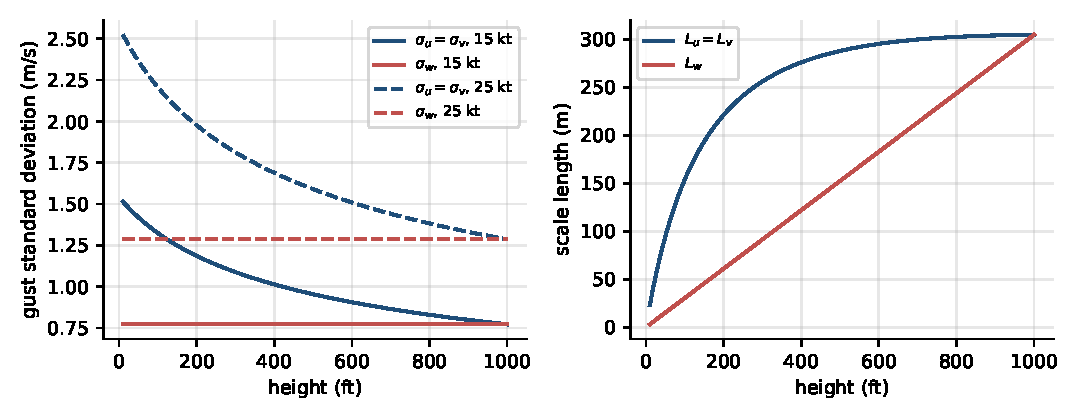
\includegraphics[width=0.92\textwidth]{dryden_params.pdf}
\caption{Dryden low-altitude parameters as implemented in
\code{dryden\_low\_altitude}. The scale lengths do not depend on the wind
speed.}
\label{fig:dryden}
\end{figure}

\subsection{Exact discretisation}

A naive Euler--Maruyama step of \eqref{eq:ou} is only accurate for
$\Delta t\ll L/V$, and at low height $L_w/V$ can be well under a second. The
code uses the exact solution of the linear SDE over one step instead:
\begin{equation}
g_{k+1} = a\,g_k + \sigma\sqrt{1-a^2}\;\xi_k,
\qquad a = e^{-V\Delta t/L},\qquad \xi_k\sim\mathcal{N}(0,1). \label{eq:oudisc}
\end{equation}
Taking the variance of both sides,
$\operatorname{Var}(g_{k+1}) = a^2\operatorname{Var}(g_k)+\sigma^2(1-a^2)$,
whose fixed point is $\sigma^2$ for \emph{any} $\Delta t$. The update is
therefore unconditionally stable and reproduces the correct variance and
autocovariance $\sigma^2a^{m}$ at lag $m$ (Figure~\ref{fig:ou}).

\begin{figure}[H]
\centering
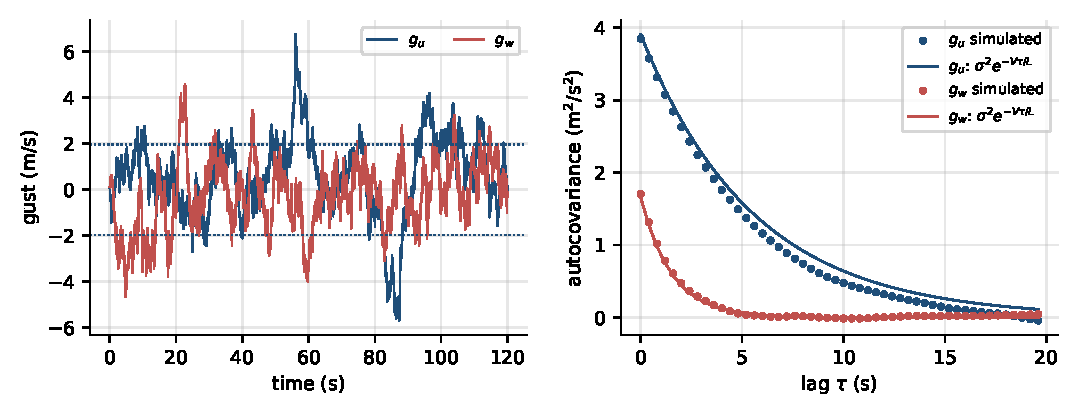
\includegraphics[width=0.92\textwidth]{ou_sample.pdf}
\caption{Left: sample gusts from \code{Turbulence.step} ($25\un{kt}$ wind,
$h=200\un{ft}$, $V=40\un{m/s}$); the dotted lines are $\pm\sigma_u$. The
vertical gust is weaker and decorrelates faster. Right: the simulated
autocovariance matches $\sigma^2e^{-V\tau/L}$.}
\label{fig:ou}
\end{figure}

\subsection{How the simulation uses it}

At each step \code{sim.py} calls the turbulence model with the current height
and the speed
\begin{equation}
V = \max\bigl(\lVert\mathbf{v}\rVert + W,\ 5\un{m/s}\bigr),
\end{equation}
where $W$ is the mean wind speed. The floor keeps the correlation time finite
in the hover. The three components use independent normal draws from a seeded
generator (NumPy \code{default\_rng(seed)}), so a run is reproducible.

\begin{codemap}
\code{wind.py}: the function \code{dryden\_low\_altitude} returns
$(\sigma_u,\sigma_w,L_u,L_w)$ in SI units, and \code{Turbulence.step} applies
\eqref{eq:oudisc} to $(g_u,g_v,g_w)$.
\end{codemap}

\begin{devnote}
\begin{itemize}[leftmargin=1.2em]
\item \textbf{Airspeed proxy.} $\lVert\mathbf v\rVert+W$ is correct on the
final (flying into the wind) and in the hover, and overestimates the airspeed
on the downwind leg, where it should be closer to $\lVert\mathbf v\rVert-W$.
The effect is a shorter gust correlation time than the physical one on that
leg; the variance is unaffected.
\item \textbf{Order of the filters.} The full Dryden model uses first-order
filters for $g_u$ and second-order filters for $g_v$ and $g_w$. Here all
three are first order, with the correct variances and scale lengths.
\item \textbf{Varying coefficients.} $\sigma$ and $L$ change with height at
every step, while \eqref{eq:oudisc} is exact for constant coefficients. During
the descent the variance of $g$ tracks $\sigma^2(h)$ with a delay of the order
of $L/V$, which is short compared with the descent.
\end{itemize}
\end{devnote}

% =====================================================================
\section{Geometry of the pattern}\label{sec:geometry}

The pattern is fixed by four numbers computed once, when the mode is created.
Let $V_g=60\un{kt}=30.87\un{m/s}$ be the gate speed and
$a=1.2\un{kt/s}=0.617\un{m/s^2}$ the deceleration.

\begin{enumerate}
\item \textbf{Hover point.} A distance $d_h=100\un{m}$ downwind of the target:
$\mathbf{p}_h=(0,-d_h)$. The aircraft stops short of the survivor so that the
survivor stays in view ahead of the nose.
\item \textbf{Reversal radius.} The radius of a coordinated turn at the gate
speed with bank $\phi_r=20^\circ$ (Annex~\ref{app:turn}):
\begin{equation}
R = \frac{V_g^2}{g\tan\phi_r} = 266.9\un{m}.
\end{equation}
\item \textbf{Downwind track.} A line parallel to the final course, offset by
one turn diameter: $x = 2\,\sigma_s R = \pm533.9\un{m}$, where
$\sigma_s=\pm1$ is the side. A semicircle of radius $R$ started on this line
ends exactly on the final course $x=0$.
\item \textbf{Length of the final.} The distance needed to stop from the gate
speed at constant deceleration (Annex~\ref{app:kin}), plus a straight margin
of $t_m=15\un{s}$ flown at the gate speed:
\begin{equation}
\ell_f = \frac{V_g^2}{2a} + V_g\,t_m = 771.7 + 463.0 = 1234.7\un{m}.
\end{equation}
The reversal starts when the aircraft, on the downwind track, passes
\begin{equation}
y_r = -d_h - \ell_f = -1334.7\un{m}.
\end{equation}
\end{enumerate}

The side is chosen at the end of the Mark phase: $\sigma_s=+1$ if $x\ge-1\un{m}$
and $-1$ otherwise. The aircraft therefore flies the pattern on the side
towards which it was already moving when the target was marked.

\begin{figure}[H]
\centering
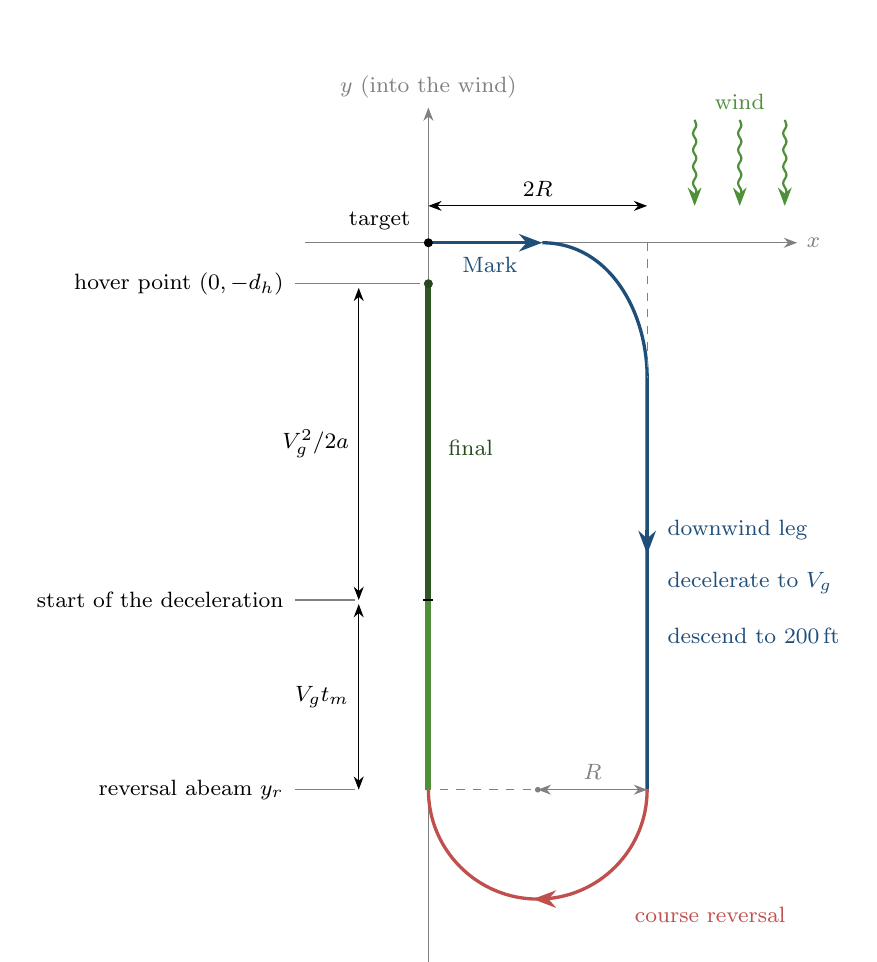
\begin{tikzpicture}[>=Stealth,x=0.0052cm,y=0.0052cm,every node/.style={font=\footnotesize}]
% axes
\draw[->,gray] (-300,0) -- (900,0) node[right]{$x$};
\draw[->,gray] (0,-1780) -- (0,330) node[above]{$y$ (into the wind)};
% final decel portion
\draw[leaf,line width=2.2pt] (0,-1335) -- (0,-872);
\draw[leaf!60!black,line width=2.2pt] (0,-872) -- (0,-100);
% track
\draw[navy,very thick,->] (0,0) -- (278,0);
\draw[navy,very thick] (278,0) to[out=0,in=90] (534,-330) -- (534,-1335);
\draw[navy,very thick,->] (534,-700) -- (534,-760);
\draw[brick,very thick] (534,-1335) arc (0:-180:267);
\draw[brick,very thick,->] (267,-1602) -- (255,-1602);
\draw[dashed,gray] (534,-1335) -- (0,-1335);
\draw[dashed,gray] (534,0) -- (534,-330);
\fill[gray] (267,-1335) circle (7);
\draw[<->,gray] (267,-1335) -- node[above]{$R$} (534,-1335);
% points
\fill (0,0) circle (11) node[above left=1pt and 3pt]{target};
\fill[leaf!50!black] (0,-100) circle (11);
\node[left] at (-330,-100) {hover point $(0,-d_h)$};
\draw[gray,thin] (-325,-100) -- (-20,-100);\draw[gray,thin] (-325,-872) -- (-180,-872);\draw[gray,thin] (-325,-1335) -- (-180,-1335);
\draw (-12,-872) -- (12,-872);
\node[left] at (-330,-872) {start of the deceleration};
\node[left] at (-330,-1335) {reversal abeam $y_r$};
\draw[<->] (-170,-872) -- node[left]{$V_g^2/2a$} (-170,-110);
\draw[<->] (-170,-1335) -- node[left]{$V_g t_m$} (-170,-882);
\draw[<->] (0,90) -- node[above]{$2R$} (534,90);
% labels
\node[navy,right] at (560,-700) {downwind leg};
\node[navy,right] at (560,-830) {decelerate to $V_g$};
\node[navy,right] at (560,-960) {descend to $200\un{ft}$};
\node[brick,right] at (480,-1640) {course reversal};
\node[leaf!50!black,right] at (25,-500) {final};
\node[navy,below] at (150,-10) {Mark};
% wind
\foreach \k in {650,760,870}
  \draw[->,leaf,thick,decorate,decoration={snake,amplitude=0.6pt,segment length=6pt,post length=3pt}] (\k,300) -- (\k,90);
\node[leaf] at (760,345) {wind};
\end{tikzpicture}
\caption{Nominal pattern in the wind-aligned frame for $\sigma_s=+1$, drawn to
scale with the default parameters. Blue: Mark and the downwind part of
Approach~1. Red: course reversal. Green: the final, which belongs to
Approach~1 until the capture conditions hold and to Approach~2 afterwards.}
\label{fig:pattern}
\end{figure}

\begin{codemap}
\code{guidance.py}: \code{MarkOnTarget.\_\_init\_\_} computes \code{r\_rev} ($R$),
\code{hover\_point} ($\mathbf p_h$) and \code{y\_reversal} ($y_r$).
\end{codemap}

% =====================================================================
\section{Guidance laws and mode logic}\label{sec:guidance}

\subsection{The state machine}

The mode has four phases; Approach~1 has three lateral sub-modes
(Figure~\ref{fig:fsm}). Transitions are evaluated at the start of every step,
before the command is computed. Table~\ref{tab:transitions} lists the exact
conditions.

\begin{figure}[H]
\centering
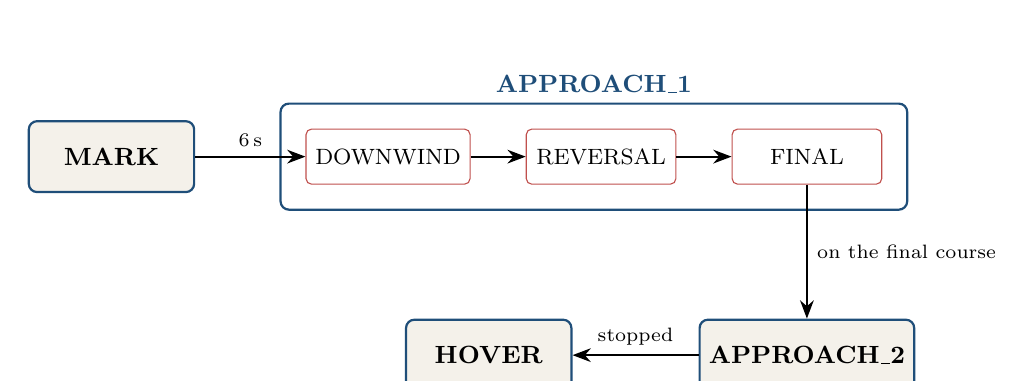
\begin{tikzpicture}[>=Stealth,node distance=0.9cm,
  ph/.style={draw=navy,thick,rounded corners=3pt,fill=sand,minimum height=0.9cm,minimum width=2.1cm,font=\small\bfseries},
  sub/.style={draw=brick,rounded corners=2pt,fill=white,minimum height=0.7cm,minimum width=1.9cm,font=\footnotesize}]
\node[ph] (mark) {MARK};
\node[sub,right=1.4cm of mark] (dw) {DOWNWIND};
\node[sub,right=0.7cm of dw] (rev) {REVERSAL};
\node[sub,right=0.7cm of rev] (fin) {FINAL};
\node[ph,below=1.7cm of fin] (a2) {APPROACH\_2};
\node[ph,left=1.6cm of a2] (hov) {HOVER};
\node[draw=navy,thick,rounded corners=3pt,fit=(dw)(rev)(fin),inner sep=9pt,label={[font=\small\bfseries,navy]above:APPROACH\_1}] (a1) {};
\draw[->,thick] (mark) -- node[above,font=\scriptsize]{$6\un{s}$} (dw);
\draw[->,thick] (dw) -- (rev);
\draw[->,thick] (rev) -- (fin);
\draw[->,thick] (fin) -- node[right,font=\scriptsize]{on the final course} (a2);
\draw[->,thick] (a2) -- node[above,font=\scriptsize]{stopped} (hov);
\end{tikzpicture}
\caption{Phases (\code{Phase}) and lateral sub-modes (\code{Lateral}) of the
Mark on Target mode.}
\label{fig:fsm}
\end{figure}

\begin{table}[H]
\centering\small
\begin{tabular}{@{}p{4.9cm}p{9.6cm}@{}}
\toprule
Transition & Condition \\
\midrule
MARK $\to$ DOWNWIND & time in phase $\ge 6\un{s}$ \\
DOWNWIND $\to$ REVERSAL & $|x-2\sigma_sR|<40\un{m}$ \ and \ $|\wrap(\psi+\pi/2)|<15^\circ$ \ and \ $y\le y_r$ \\
REVERSAL $\to$ FINAL & $|\wrap(\psi-\pi/2)|<10^\circ$ \\
FINAL $\to$ APPROACH\_2 & $|x|<15\un{m}$ \ and \ $|\wrap(\psi-\pi/2)|<5^\circ$ \\
APPROACH\_2 $\to$ HOVER & $\lVert\mathbf p_h-\mathbf p\rVert<5\un{m}$ \ and \ $V<0.5\un{m/s}$ \ and \ $|h-50|<3\un{ft}$ \\
\bottomrule
\end{tabular}
\caption{Transition conditions in \code{MarkOnTarget.\_transitions}.}
\label{tab:transitions}
\end{table}

\subsection{Line tracking: the L1-style law}\label{sec:l1}

Two straight lines are tracked: the downwind track and the final course. For a
line through $\mathbf p_0$ with unit direction $\mathbf d$, the signed
cross-track error is the 2D cross product
\begin{equation}
e = d_x\,(y-y_0) - d_y\,(x-x_0), \qquad e>0 \text{ when the aircraft is left of the line,}
\end{equation}
and the commanded heading is the direction of the line, corrected towards it:
\begin{equation}
\psi_c = \wrap\!\Bigl(\operatorname{atan2}(d_y,d_x) - \arctan\frac{e}{L_1}\Bigr),
\qquad L_1=400\un{m}. \label{eq:l1}
\end{equation}
Geometrically the aircraft aims at a point on the line a distance $L_1$ ahead
of its own projection (Figure~\ref{fig:l1}, left). Far from the line
($|e|\gg L_1$) the intercept angle tends to $90^\circ$; close to it the
correction is proportional to the error.

\textbf{Dynamics of the capture.} If the heading follows the command and the
speed is $V$, the cross-track error obeys
\begin{equation}
\dot e = V\sin\Bigl(-\arctan\frac{e}{L_1}\Bigr) = -\frac{V\,e}{\sqrt{L_1^2+e^2}}
\;\;\approx\;\; -\frac{V}{L_1}\,e \quad (|e|\ll L_1).
\end{equation}
The error decreases monotonically for any initial condition, at a rate that is
at most $V$, and close to the line it decays exponentially with time constant
$L_1/V$: $13\un{s}$ at $60\un{kt}$ and $8.6\un{s}$ at $90\un{kt}$
(Figure~\ref{fig:l1}, right). $L_1$ is the single tuning parameter: a smaller
value captures faster, but once $L_1/V$ approaches the response time of the
heading channel the neglected turn dynamics produce overshoot.

\begin{figure}[H]
\centering
\begin{minipage}{0.42\textwidth}
\centering
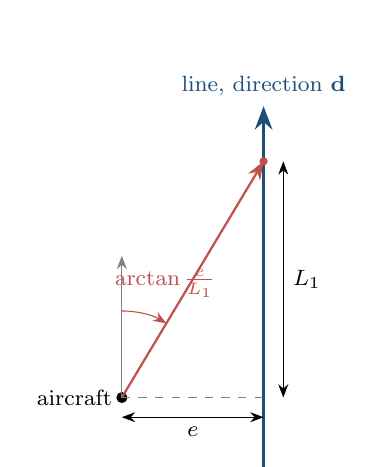
\begin{tikzpicture}[>=Stealth,scale=1.0,every node/.style={font=\footnotesize}]
\draw[navy,very thick,->] (0,-0.4) -- (0,4.3) node[above]{line, direction $\mathbf d$};
\fill (-1.8,0.6) circle (2pt) node[left]{aircraft};
\draw[dashed,gray] (-1.8,0.6) -- (0,0.6);
\draw[<->] (-1.8,0.35) -- node[below]{$e$} (0,0.35);
\draw[<->] (0.25,0.6) -- node[right]{$L_1$} (0.25,3.6);
\draw[brick,thick,->] (-1.8,0.6) -- (0,3.6);
\draw[gray,->] (-1.8,0.6) -- (-1.8,2.4);
\draw[brick,->] (-1.8,1.7) arc (90:59:1.1);
\node[brick] at (-1.25,2.05) {$\arctan\frac{e}{L_1}$};
\fill[brick] (0,3.6) circle (1.5pt);
\end{tikzpicture}
\end{minipage}\hfill
\begin{minipage}{0.55\textwidth}
\centering
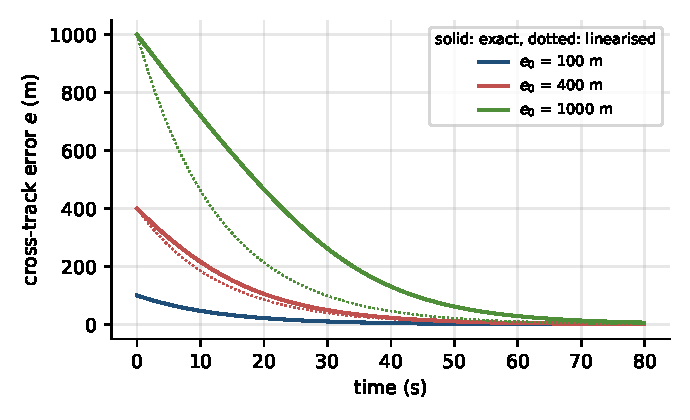
\includegraphics[width=\textwidth]{l1_capture.pdf}
\end{minipage}
\caption{Left: geometry of the law \eqref{eq:l1}. Right: capture from three
initial offsets at $60\un{kt}$ with an ideal heading response.}
\label{fig:l1}
\end{figure}

\subsection{The height loop}\label{sec:height}

In every phase the vertical command has the same structure: a reference height
$h_{\text{ref}}$, a proportional term and, while descending, a feed-forward of
the scheduled rate $\dot h_s=200\un{ft/min}=3.33\un{ft/s}$:
\begin{equation}
\dot h_c = \max\bigl(\dot h_{\text{ff}} + k_h\,(h_{\text{ref}}-h),\ -\dot h_s\bigr),
\qquad k_h=0.5\un{s^{-1}}, \label{eq:hloop}
\end{equation}
with $\dot h_{\text{ff}}=-\dot h_s$ while the reference is ramping down and
$0$ otherwise. Together with the lag \eqref{eq:vert} the closed loop is of
second order,
\begin{equation}
\tau_h\,\ddot h + \dot h + k_h\,h = k_h\,h_{\text{ref}}
\;\;\Longrightarrow\;\;
\omega_n=\sqrt{k_h/\tau_h}=0.707\un{rad/s},\quad
\zeta=\frac{1}{2\sqrt{k_h\tau_h}}=0.707,
\end{equation}
a well damped response with about $4\%$ overshoot
(Annex~\ref{app:second}, Figure~\ref{fig:steps}).

\textbf{Effect of the clamp.} The $\max(\cdot,-\dot h_s)$ guarantees that the
commanded descent never exceeds the schedule. It also disables the
proportional term whenever the aircraft is \emph{above} the ramping reference.
The aircraft takes about $\tau_h$ to reach the scheduled rate, falls behind
the reference by $\dot h_s\tau_h\approx3.3\un{ft}$, and keeps that offset
until the ramp ends and the loop closes it. This is why Approach~2 ends about
$3\un{ft}$ high (Figure~\ref{fig:a2}) and why the transition to the hover
allows $\pm3\un{ft}$.

\subsection{Phase MARK}

For $6\un{s}$ the mode holds what the aircraft was doing at the mark:
\begin{equation}
\mathbf v_c = V_{\text{ref}}\,(\cos\psi,\sin\psi),\qquad
\psi_c=\psi_{\text{hold}},\qquad
\dot h_c = k_h(h_{\text{ref}}-h),
\end{equation}
with $V_{\text{ref}}$, $\psi_{\text{hold}}$ and $h_{\text{ref}}$ frozen at the
initial state (radar-altitude hold). The target is the origin of the frame, so
``storing the target'' needs no code.

\subsection{Phase APPROACH\_1}

\textbf{Speed.} The reference is ramped down at the scheduled deceleration to
the gate speed, and commanded along the nose:
\begin{equation}
V_{\text{ref}} \leftarrow \max(V_{\text{ref}}-a\,\Delta t,\ V_g),
\qquad \mathbf v_c = V_{\text{ref}}\,(\cos\psi,\sin\psi).
\end{equation}
Because the velocity command follows the heading, the heading channel steers
the aircraft and the turn is flown as a turn: there is no sideslip between
heading and track beyond the lag $\tau_v$. From $90\un{kt}$ the ramp takes
$25\un{s}$.

\textbf{Height.} The reference ramps from the entry height to the gate height
of $200\un{ft}$ at $\dot h_s$, with the command \eqref{eq:hloop}. From
$500\un{ft}$ this takes $90\un{s}$, so the descent is the slowest element of
Approach~1.

\textbf{Lateral sub-modes.}
\begin{itemize}
\item \emph{DOWNWIND}: track the line through $(2\sigma_sR,0)$ with direction
$(0,-1)$ using \eqref{eq:l1}.
\item \emph{REVERSAL}: a turn of fixed \emph{radius}. The heading command leads
the current heading by a constant $0.6\un{rad}$ towards the final course, and
the turn rate is limited to
\begin{equation}
\psi_c = \wrap(\psi - 0.6\,\sigma_s), \qquad
r_{\lim} = \frac{V}{R_t}, \qquad
R_t = \max\!\bigl(|x|/2,\ R/2\bigr).
\end{equation}
Since $k_\psi\cdot0.6=0.9\un{rad/s}$ is far above $r_{\lim}$, the heading
channel is saturated and the aircraft turns at exactly $V/R_t$, that is, on a
circle of radius $R_t$ whatever the speed. $R_t$ is fixed at the start of the
reversal as half the actual distance to the final course, so that the
semicircle ends on $x=0$ even if the aircraft was a few metres off the
downwind track. Nominally $R_t\approx R$: a turn at
$6.6^\circ/\mathrm{s}$ that lasts $\pi R/V_g=27\un{s}$.
\item \emph{FINAL}: track the line through the origin with direction $(0,1)$
using \eqref{eq:l1}, until the capture conditions of
Table~\ref{tab:transitions} hold.
\end{itemize}

\begin{devnote}
\begin{itemize}[leftmargin=1.2em]
\item The limit $r_{\lim}$ \emph{replaces} the bank limit \eqref{eq:rmax}. The
equivalent bank is $\tan\phi=V^2/(gR_t)$: $20^\circ$ at the gate speed, but
$39^\circ$ if the reversal were entered at $90\un{kt}$. With the default
parameters the gate speed is always reached first; a shorter pattern or a
higher entry speed can break that.
\item The transition to Approach~2 checks position and heading only. It does
not check that the gate speed and the gate height have been reached. The
Approach~2 laws tolerate this (they take over from the current
$V_{\text{ref}}$ and $h_{\text{ref}}$), but the name ``gate'' is then nominal.
\end{itemize}
\end{devnote}

\subsection{Phase APPROACH\_2}

This is the core of the manoeuvre: decelerate and descend so that groundspeed
and height reach their hover values at the same moment, over the hover point.

\textbf{Speed profile.} Let $d=\max(y_h-y,0)$ be the distance to go along the
final. An aircraft that decelerates at a constant $a$ and stops exactly at
$d=0$ must have, at every point (Annex~\ref{app:kin}),
\begin{equation}
V(d) = \sqrt{2\,a\,d}. \label{eq:vprofile}
\end{equation}
The code uses this curve with two refinements:
\begin{equation}
V_{\text{ref}} \leftarrow \min\!\Bigl(V_{\text{ref}},\ \sqrt{2a\,\max(d - V\,t_\ell,\,0)}\Bigr),
\qquad t_\ell = 1\un{s}.
\end{equation}
The $\min$ makes the reference non-increasing: the aircraft holds the gate
speed until it meets the curve and then follows it down. The term $V\,t_\ell$
evaluates the curve at the position the aircraft will have one response time
later, which compensates the lag $\tau_v$ so that the real aircraft does not
overshoot the hover point. Note that a feedback law of the form
\eqref{eq:vprofile} produces a constant deceleration by itself:
$\dot V = \frac{\dd V}{\dd d}\,\dot d = \frac{a}{V}(-V) = -a$.

\textbf{Time to go.} With $V$ the current speed (floored at $1\un{m/s}$), the
remaining time is a constant-speed segment followed by the deceleration:
\begin{equation}
t_{\text{go}} = \frac{\max\bigl(d - V^2/2a,\ 0\bigr)}{V} + \frac{V}{a}.
\label{eq:tgo}
\end{equation}

\textbf{Descent schedule.} The descent from $h_{\text{ref}}$ to the hover
height $h_h=50\un{ft}$ at the rate $\dot h_s$ needs a time
$(h_{\text{ref}}-h_h)/\dot h_s$. The descent is started when that time equals
the time to go:
\begin{equation}
\text{descend while}\quad h_{\text{ref}}-h_h \;\ge\; \dot h_s\,t_{\text{go}} - 1\un{ft}.
\end{equation}
While the condition holds, $h_{\text{ref}}$ ramps down and the command is
\eqref{eq:hloop} with the feed-forward. The margin of $1\un{ft}$ gives the
condition hysteresis: once the descent starts, both sides decrease at the
same rate and it does not chatter. Nominally the descent of $150\un{ft}$ takes
$45\un{s}$ and the deceleration from the gate speed $50\un{s}$, so the descent
starts about $5\un{s}$ after the deceleration.

\textbf{Lateral.} The velocity is commanded in \emph{ground axes}, not along
the nose:
\begin{equation}
\mathbf v_c = \bigl(\sat(-k_y\,x,\ \pm3\un{m/s}),\ V_{\text{ref}}\bigr),
\qquad k_y=0.05\un{s^{-1}}.
\end{equation}
With the lag $\tau_v$ the lateral error obeys $\tau_v\ddot x+\dot x+k_yx=0$,
an overdamped system with poles at $-0.053$ and $-0.947\un{s^{-1}}$: no
overshoot, and a slow time constant of $19\un{s}$. The heading is commanded
separately: the line-tracking law \eqref{eq:l1} above $15\un{kt}$, and
$\psi_c=\pi/2$ (into the wind) below. Velocity and heading are thus decoupled
at low speed, as they are in a real helicopter near the hover.

\textbf{End of the approach.} Within $3\un{m}$ of the hover point the command
switches to the position hold of the next section, while the phase stays
APPROACH\_2 until the speed and height conditions of
Table~\ref{tab:transitions} hold.

\begin{figure}[H]
\centering
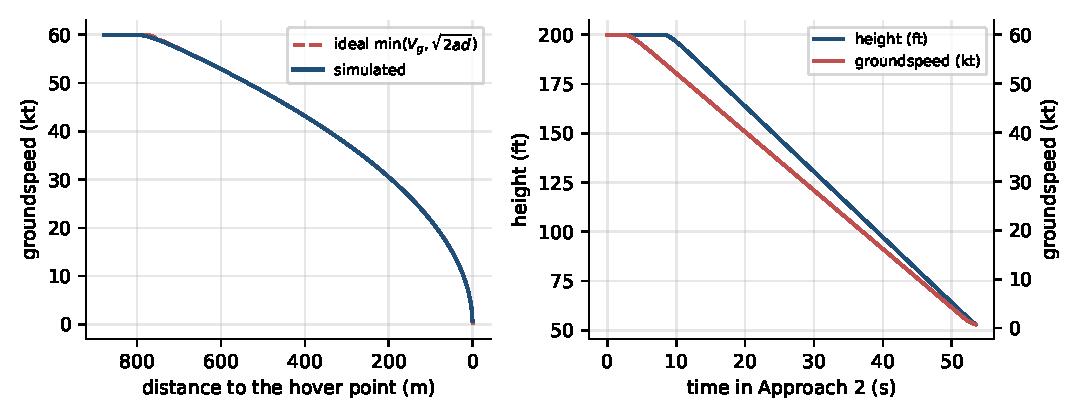
\includegraphics[width=0.95\textwidth]{approach2_profile.pdf}
\caption{Approach~2 in the default run. Left: the simulated groundspeed
follows the constant-deceleration curve, slightly inside it because of the
lead term. Right: speed and height reach the hover values together.}
\label{fig:a2}
\end{figure}

\subsection{Phase HOVER: position hold}

\begin{equation}
\mathbf v_c = \sat_{\lVert\cdot\rVert}\bigl(k_p\,(\mathbf p_h-\mathbf p),\ 3\un{m/s}\bigr),
\qquad \psi_c=\frac{\pi}{2},\qquad
\dot h_c = \sat\bigl(k_h(h_h-h),\ \pm\dot h_s\bigr),
\end{equation}
with $k_p=0.35\un{s^{-1}}$. The saturation acts on the norm of the vector.
Each horizontal axis is the same second-order system as the height loop, with
\begin{equation}
\omega_n=\sqrt{k_p/\tau_v}=0.59\un{rad/s},\qquad
\zeta=\frac{1}{2\sqrt{k_p\tau_v}}=0.85,
\end{equation}
which returns to the hover point in about $8\un{s}$ with less than $1\%$
overshoot (Figure~\ref{fig:steps}). The law is purely proportional: there is
no integral term, and none is needed because the model has no steady
disturbance (the mean wind is trimmed by assumption). In turbulence the
position error is driven by the gusts through \eqref{eq:vel}.

\begin{figure}[H]
\centering
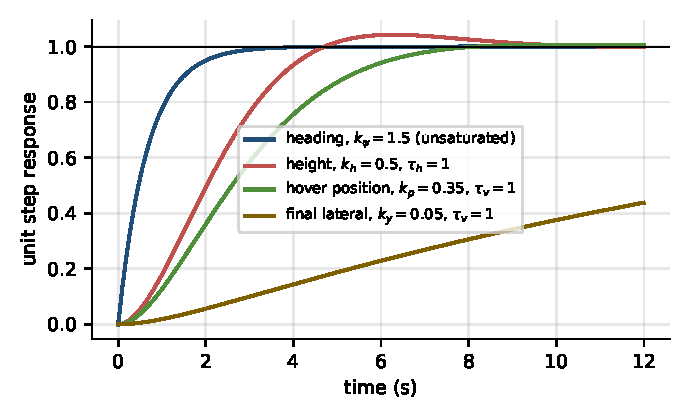
\includegraphics[width=0.6\textwidth]{step_responses.pdf}
\caption{Unit step responses of the four linear loops with the default gains.}
\label{fig:steps}
\end{figure}

\begin{codemap}
\code{guidance.py}: \code{track\_line} is \eqref{eq:l1};
\code{MarkOnTarget.update} contains the phase laws in the order of this
section; \code{\_position\_hold} is the hover law.
\end{codemap}

\begin{devnote}[Developer note: constants that are not parameters]
Several numbers are written directly in \code{guidance.py} and are not part of
\code{MOTParams}: the height gain $k_h=0.5$, the lead time $t_\ell=1.0\un{s}$
(equal to the default $\tau_v$ but not linked to it), the reversal lead of
$0.6\un{rad}$, the lateral gain $k_y=0.05$ with its $3\un{m/s}$ limit, and all
the transition tolerances of Table~\ref{tab:transitions}. If you change
$\tau_v$, review $t_\ell$, $k_p$ and $k_y$ with the damping formulas above.
\end{devnote}

% =====================================================================
\section{The simulation loop}\label{sec:loop}

\code{run\_mark\_on\_target} builds the initial state from the configuration
(aircraft over the target, at the entry heading, speed and height, with zero
vertical speed) and repeats, with $\Delta t=0.05\un{s}$:
\begin{enumerate}
\item $\mathbf c_k = \text{mode}(\mathbf s_k)$: transitions, then command;
\item $\mathbf g_k = \text{turbulence}(V_k,h_k)$, equation \eqref{eq:oudisc};
\item $\mathbf s_{k+1} = \text{helicopter}(\mathbf s_k,\mathbf c_k,\mathbf g_k)$,
Section~\ref{sec:model};
\item record time, position, height, groundspeed, true heading \eqref{eq:hdg},
vertical speed and phase.
\end{enumerate}
The loop ends after $20\un{s}$ in the HOVER phase, or at $t_{\max}=900\un{s}$
if the hover is never reached. The recorded positions are then rotated to
East/North with \eqref{eq:en}.

\begin{figure}[H]
\centering
\begin{subfigure}[b]{0.46\textwidth}
\centering
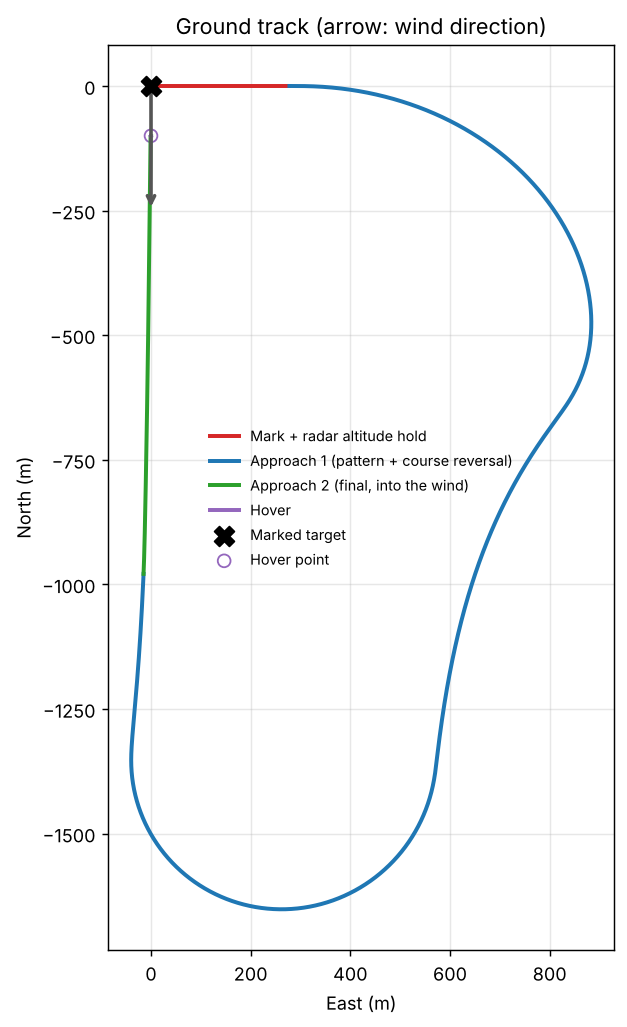
\includegraphics[height=0.3\textheight,width=\textwidth,keepaspectratio]{mot_ground_track.png}
\caption{Ground track, calm air.}
\end{subfigure}\hfill
\begin{subfigure}[b]{0.46\textwidth}
\centering
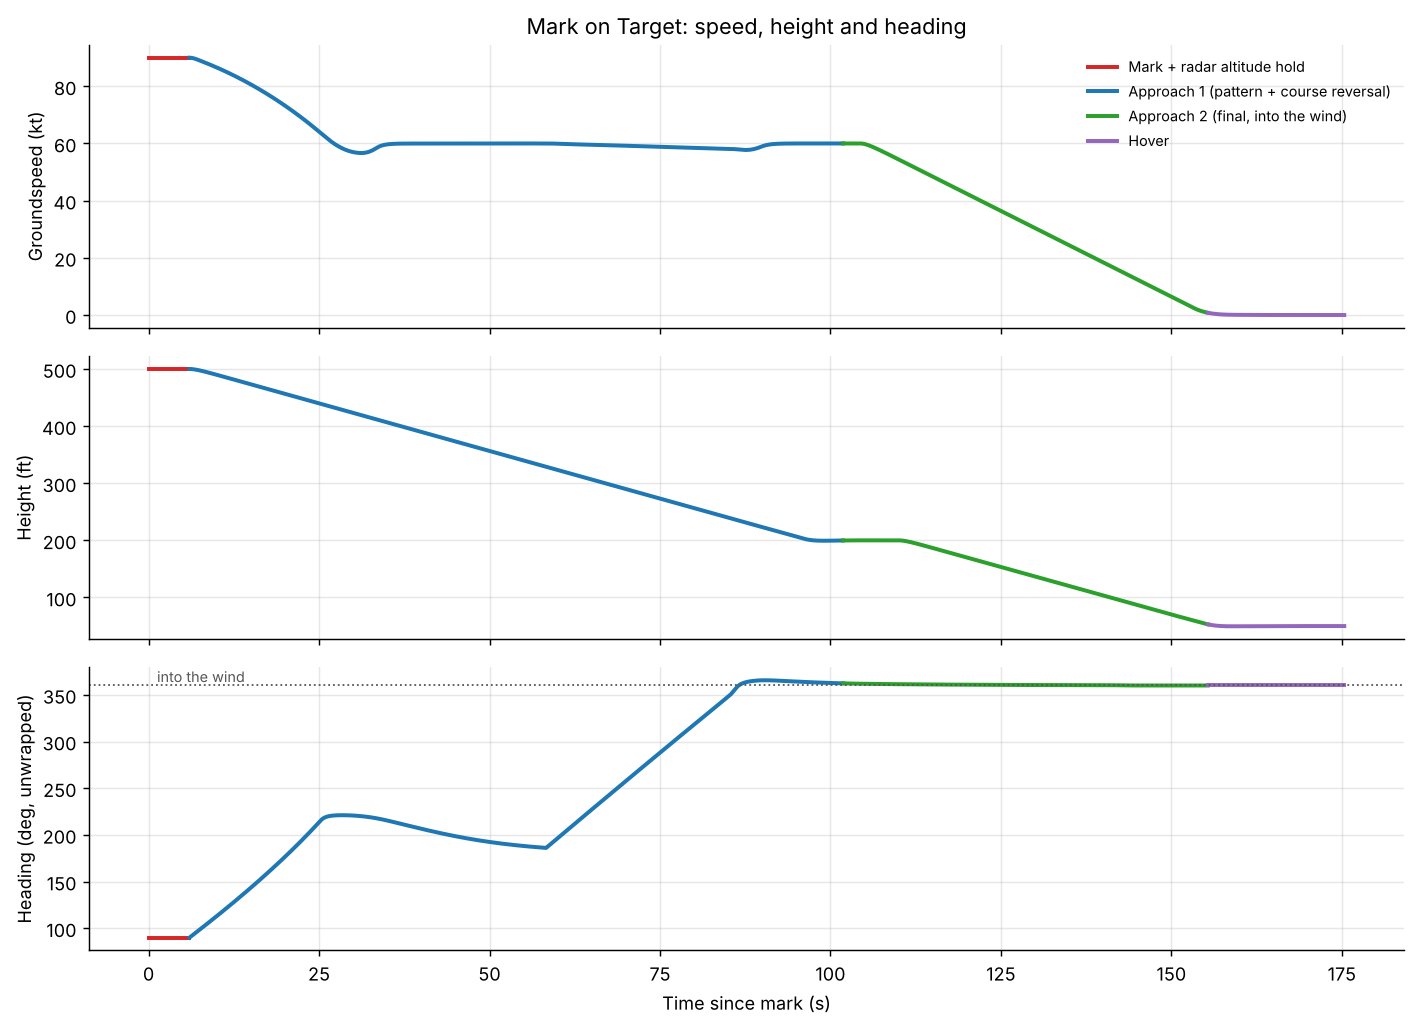
\includegraphics[width=\textwidth]{mot_profiles.png}
\caption{Speed, height and heading.}
\end{subfigure}

\vspace{0.6em}
\begin{subfigure}[b]{0.46\textwidth}
\centering
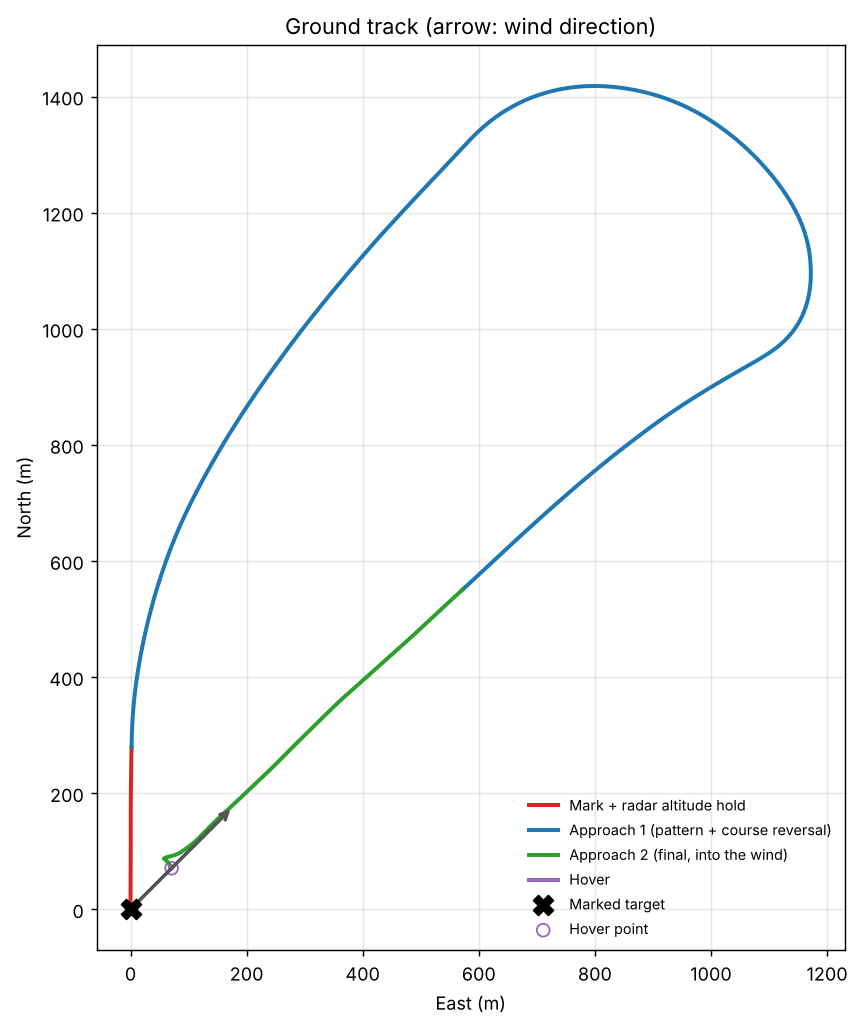
\includegraphics[height=0.3\textheight,width=\textwidth,keepaspectratio]{mot_ground_track_turbulence.png}
\caption{Ground track with turbulence.}
\end{subfigure}\hfill
\begin{subfigure}[b]{0.46\textwidth}
\centering
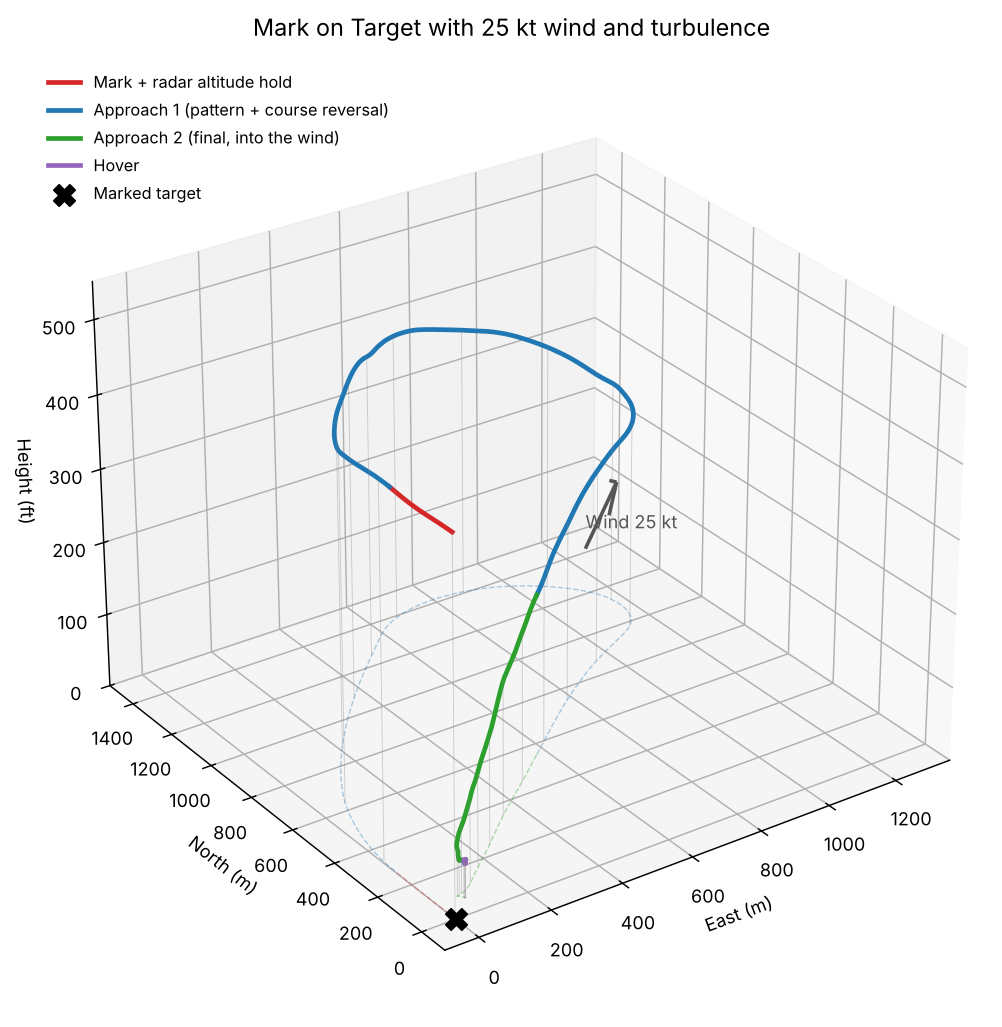
\includegraphics[width=\textwidth]{mot_3d_turbulence.png}
\caption{Trajectory with a $25\un{kt}$ wind and turbulence.}
\end{subfigure}
\caption{Output of the simulator (figures of the repository, produced by
\code{examples/reproduce\_article\_figures.py}).}
\label{fig:outputs}
\end{figure}

For the default configuration (wind $15\un{kt}$ from the north, entry heading
east at $90\un{kt}$ and $500\un{ft}$) the phases last:

\begin{table}[H]
\centering\small
\begin{tabular}{@{}lrrrr@{}}
\toprule
Phase & Start (s) & End (s) & Height at the end (ft) & Groundspeed at the end (kt) \\
\midrule
MARK & 0.0 & 6.0 & 500 & 90 \\
APPROACH\_1 & 6.0 & 101.8 & 200 & 60 \\
APPROACH\_2 & 101.9 & 155.4 & 53 & 1 \\
HOVER & 155.4 & 175.4 & 50 & 0 \\
\bottomrule
\end{tabular}
\caption{Timeline of the default run.}
\end{table}

% =====================================================================
\section{What the tests verify}\label{sec:tests}

The test suite turns the claims of this guide into assertions. When you change
a law or a gain, these are the properties that must still hold.

\begin{table}[H]
\centering\small
\begin{tabular}{@{}p{14.4cm}@{}}
\toprule
Test, property and where it comes from \\
\midrule
\code{test\_reaches\_hover\_into\_wind}\newline For several wind directions and entry
headings: in HOVER the distance to the hover point is below $3\un{m}$, the
heading is within $2^\circ$ of the wind direction and $|h-50|<5\un{ft}$.
Checks the frame conversions \eqref{eq:hdg}--\eqref{eq:en} and the whole chain. \\[0.3em]
\code{test\_phases\_in\_order}\newline The phases appear in the order of
Figure~\ref{fig:fsm}. \\[0.3em]
\code{test\_hover\_point\_is\_downwind\_of\_target}\newline With wind from the north
the hover point is exactly $100\un{m}$ south of the target
(Section~\ref{sec:geometry}). \\[0.3em]
\code{test\_approach\_2\_respects\_rates}\newline In Approach~2 the deceleration
stays below $1.2\un{kt/s}$ plus $25\%$ and the descent rate below
$200\un{ft/min}$ plus $10\%$ (speed profile \eqref{eq:vprofile} and clamp in
\eqref{eq:hloop}). \\[0.3em]
\code{test\_turbulence\_hover\_stays\_close}\newline With turbulence the hover stays
within $10\un{m}$ and $15\un{ft}$ (gust rejection of \eqref{eq:vel} and the
position hold). \\[0.3em]
\code{test\_turbulence\_statistics\_match\_dryden\_sigma}\newline The sample standard
deviation of a long gust series matches $\sigma_u$ and $\sigma_w$ within
$15\%$ (stationary variance of \eqref{eq:oudisc}). \\[0.3em]
\code{test\_csv\_export}\newline File format. \\
\bottomrule
\end{tabular}
\caption{Tests in \code{tests/test\_mark\_on\_target.py}.}
\end{table}

% =====================================================================
\section{Limits of the model and natural extensions}

The simplifications below are deliberate. They are listed so that nobody
mistakes the simulator for something it is not, and as a map of where the
physics can be deepened.

\begin{enumerate}
\item \textbf{No air mass.} The ground velocity is controlled directly; the
mean wind does not drift the aircraft and the power, attitude and airspeed
effects of the wind are absent. \emph{Extension:} carry
$\mathbf v_{\text{air}}$ as the state and add the wind vector.
\item \textbf{No attitude dynamics.} Bank and pitch do not exist as states;
the bank only appears as a turn-rate limit. \emph{Extension:} add a bank state
with its own lag, so that roll-in and roll-out take time.
\item \textbf{Decoupled channels.} Turning, accelerating and climbing do not
compete for power or for rotor thrust.
\item \textbf{Simplified turbulence.} First-order filters on all axes, gusts
expressed in wind axes, an airspeed proxy that ignores the direction of
flight, and no gust gradients (no rotational gusts).
\item \textbf{Ideal sensors.} The guidance uses the true state: no radar
altimeter noise, no Doppler or GPS velocity error, no delay.
\item \textbf{Proportional loops only.} Without steady disturbances no
integral action is needed. It will be once a real wind is added.
\end{enumerate}

\newpage
\appendix
% =====================================================================
\section{Prerequisites: vectors, rotations and angles}\label{app:vec}

\textbf{Vectors.} A point or a velocity in the plane is a pair
$\mathbf v=(v_x,v_y)$ with norm $\lVert\mathbf v\rVert=\sqrt{v_x^2+v_y^2}$
(\code{np.hypot}). The unit vector of direction $\psi$ is
$(\cos\psi,\sin\psi)$.

\textbf{Dot and cross products.} For $\mathbf a$ and $\mathbf b$ in the plane,
\[
\mathbf a\cdot\mathbf b = a_xb_x+a_yb_y = \lVert\mathbf a\rVert\lVert\mathbf b\rVert\cos\theta,
\qquad
\mathbf a\times\mathbf b = a_xb_y-a_yb_x = \lVert\mathbf a\rVert\lVert\mathbf b\rVert\sin\theta,
\]
where $\theta$ is the angle from $\mathbf a$ to $\mathbf b$,
counter-clockwise. If $\mathbf a$ is a unit vector along a line and
$\mathbf b$ goes from a point of the line to the aircraft, $\mathbf a\cdot\mathbf b$
is the distance \emph{along} the line and $\mathbf a\times\mathbf b$ the signed
distance \emph{across} it, positive to the left. This is the cross-track error
of Section~\ref{sec:l1}.

\textbf{Rotations.} The matrix
$\begin{psmallmatrix}\cos\theta&-\sin\theta\\ \sin\theta&\cos\theta\end{psmallmatrix}$
rotates a vector by $\theta$ counter-clockwise. Compass bearings grow
clockwise, which is why the matrix in \eqref{eq:en} has the signs of a
rotation by $-\beta$.

\textbf{atan2.} $\operatorname{atan2}(y,x)$ returns the angle of the vector
$(x,y)$ in $(-\pi,\pi]$, with the correct quadrant, unlike $\arctan(y/x)$.

\textbf{Two angle conventions.} Mathematics measures angles from $+x$,
counter-clockwise. Navigation measures headings from North, clockwise. For a
frame with $x$ east and $y$ north the conversion is
$\psi=90^\circ-\chi$; equation \eqref{eq:hdg} is the same relation in a frame
rotated by $\beta$.

% =====================================================================
\section{Prerequisites: first-order systems and numerical integration}\label{app:first}

\textbf{The first-order lag.} The equation
\begin{equation}
\tau\,\dot x + x = u
\end{equation}
describes a quantity $x$ that follows its command $u$ with a delay. For a
constant $u$ and $x(0)=x_0$ the solution is
\[
x(t) = u + (x_0-u)\,e^{-t/\tau}.
\]
The \emph{time constant} $\tau$ is the time to cover $63\%$ of a step; after
$3\tau$ the response is within $5\%$. For a ramp command $u=ct$ the output
follows the ramp with a constant delay $\tau$, that is, an error $c\,\tau$:
this is the $3.3\un{ft}$ of Section~\ref{sec:height} and the reason for the
lead term in the speed profile.

\textbf{Transfer function.} In the Laplace domain the lag is
$G(s)=\dfrac{1}{\tau s+1}$, with one pole at $s=-1/\tau$. A proportional loop
around a pure integrator, $\dot x=k(u-x)$, is the same system with $\tau=1/k$;
this is the heading channel \eqref{eq:heading}.

\textbf{Saturation.} $\sat(z,\pm m)=\max(-m,\min(m,z))$ (\code{np.clip}). A
loop in saturation moves at its limit rate and behaves linearly only once the
error is small. For vectors the code scales the whole vector to the limit norm.

\textbf{Explicit Euler.} $x_{k+1}=x_k+f(x_k)\,\Delta t$ approximates
$\dot x=f(x)$ with a local error proportional to $\Delta t^2$. Applied to the
lag it gives $x_{k+1}=(1-\Delta t/\tau)x_k+(\Delta t/\tau)u$, stable for
$\Delta t<2\tau$. Rule of thumb: keep $\Delta t\le\tau/10$ for the fastest
time constant of the model.

% =====================================================================
\section{Prerequisites: second-order systems and feedback}\label{app:second}

Closing a proportional position loop of gain $k$ around a velocity lag $\tau$
gives the structure that appears three times in the simulator (height, hover
position, lateral position on the final):
\begin{equation}
\dot x = v,\quad \tau\dot v + v = k\,(x_{\text{ref}}-x)
\;\;\Longrightarrow\;\;
\ddot x + \frac{1}{\tau}\dot x + \frac{k}{\tau}x = \frac{k}{\tau}x_{\text{ref}} .
\end{equation}
Comparing with the standard form
$\ddot x+2\zeta\omega_n\dot x+\omega_n^2x=\omega_n^2x_{\text{ref}}$:
\begin{equation}
\omega_n=\sqrt{\frac{k}{\tau}},\qquad \zeta=\frac{1}{2\sqrt{k\,\tau}} .
\end{equation}
The \emph{natural frequency} $\omega_n$ sets the speed of the response and the
\emph{damping ratio} $\zeta$ its shape:
\begin{itemize}
\item $\zeta<1$ (underdamped): oscillatory, overshoot
$\exp\bigl(-\pi\zeta/\sqrt{1-\zeta^2}\bigr)$; $4.3\%$ for $\zeta=0.707$;
\item $\zeta=1$ (critically damped): the fastest response without overshoot,
obtained for $k=1/(4\tau)$;
\item $\zeta>1$ (overdamped): two real poles, one of them slow.
\end{itemize}
The design rule that follows is simple: for a given inner lag $\tau$, raising
the outer gain $k$ makes the loop faster and less damped. Gains above
$1/(2\tau)$ give $\zeta<0.707$ and visible overshoot.

\begin{table}[H]
\centering\small
\begin{tabular}{@{}lrrrr@{}}
\toprule
Loop & $k$ (s$^{-1}$) & $\tau$ (s) & $\omega_n$ (rad/s) & $\zeta$ \\
\midrule
Height & 0.50 & 1.0 & 0.71 & 0.71 \\
Hover position & 0.35 & 1.0 & 0.59 & 0.85 \\
Lateral on the final & 0.05 & 1.0 & 0.22 & 2.24 \\
\bottomrule
\end{tabular}
\caption{The three second-order loops with the default parameters.}
\end{table}

\textbf{Feed-forward.} When the reference moves in a known way (a ramp), the
known rate can be added directly to the command instead of waiting for an
error to build up. In \eqref{eq:hloop} the scheduled descent rate is the
feed-forward and the proportional term only corrects what is left.

% =====================================================================
\section{Prerequisites: kinematics at constant acceleration}\label{app:kin}

A body that moves along a line with constant deceleration $a$ from speed
$V_0$ satisfies
\[
V(t)=V_0-a\,t,\qquad s(t)=V_0t-\tfrac12at^2 .
\]
Eliminating time gives the relation between speed and distance,
$V^2=V_0^2-2as$. Two results follow:
\begin{align}
\text{time to stop:}\quad & t_s = \frac{V_0}{a}, &
\text{distance to stop:}\quad & d_s=\frac{V_0^2}{2a}.
\end{align}
Read backwards, the speed an aircraft must have at a distance $d$ from the
point where it wants to stop is $V=\sqrt{2ad}$, which is the profile
\eqref{eq:vprofile}. From $60\un{kt}$ at $1.2\un{kt/s}$: $t_s=50\un{s}$ and
$d_s=772\un{m}$.

The time to go \eqref{eq:tgo} is the same idea in two segments: the distance
beyond $d_s$ is flown at constant speed, the rest while decelerating.

% =====================================================================
\section{Prerequisites: the physics of a level turn}\label{app:turn}

In a level, coordinated turn the rotor thrust $T$ is tilted by the bank angle
$\phi$. Its vertical component balances the weight and its horizontal
component is the centripetal force (Figure~\ref{fig:turn}):
\begin{equation}
T\cos\phi = m\,g,\qquad T\sin\phi = \frac{m\,V^2}{R} .
\end{equation}
Dividing the two equations eliminates the thrust and the mass:
\begin{equation}
\tan\phi=\frac{V^2}{g\,R}
\quad\Longrightarrow\quad
R=\frac{V^2}{g\tan\phi},\qquad
\dot\psi=\frac{V}{R}=\frac{g\tan\phi}{V}. \label{eq:turn}
\end{equation}
For a given bank, the radius grows with the \emph{square} of the speed and the
turn rate falls with the speed. This is why the pattern is sized with the gate
speed and why the reversal is flown after the deceleration. The load factor is
$n=T/(mg)=1/\cos\phi$: $1.06$ at $20^\circ$ and $1.10$ at $25^\circ$.

Strictly, $V$ in \eqref{eq:turn} is the airspeed and the circle is drawn in
the air mass, which drifts with the wind. The simulator uses the groundspeed
(Section~\ref{sec:model}).

\begin{figure}[H]
\centering
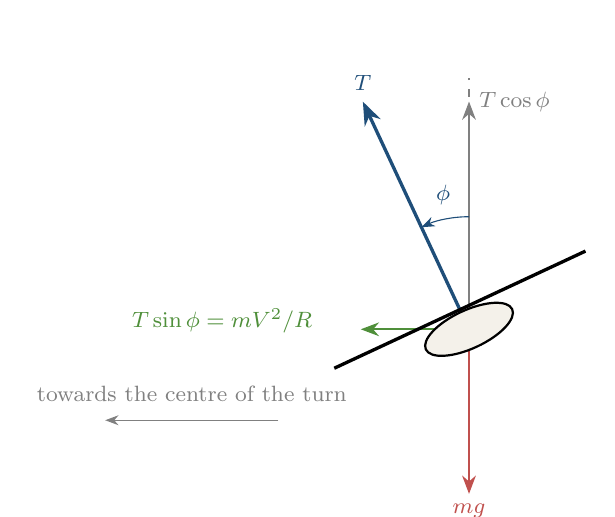
\begin{tikzpicture}[>=Stealth,scale=1.1,every node/.style={font=\footnotesize}]
\draw[gray,dashed] (0,0) -- (0,2.9);
\draw[->,very thick,navy] (0,0) -- (115:2.9) node[above]{$T$};
\draw[->,thick,brick] (0,0) -- (0,-1.9) node[below]{$mg$};
\draw[->,thick,leaf] (0,0) -- (-1.25,0);
\node[leaf,left] at (-1.7,0.1) {$T\sin\phi = mV^2/R$};
\draw[->,thick,gray] (0,0) -- (0,2.63) node[right]{$T\cos\phi$};
\draw[navy,->] (0,1.3) arc (90:115:1.3);
\node[navy] at (-0.3,1.55) {$\phi$};
\begin{scope}[rotate=25]
\draw[very thick] (-1.6,0.25) -- (1.6,0.25);
\draw[fill=sand,thick] (0,0) ellipse (0.55 and 0.22);
\end{scope}
\node[gray] at (-3.2,-0.75) {towards the centre of the turn};
\draw[gray,->] (-2.2,-1.05) -- (-4.2,-1.05);
\end{tikzpicture}
\caption{Forces in a level coordinated turn, seen from behind.}
\label{fig:turn}
\end{figure}

% =====================================================================
\section{Prerequisites: random processes}\label{app:stoch}

\textbf{Gaussian variables.} $\xi\sim\mathcal N(\mu,\sigma^2)$ has mean $\mu$
and variance $\sigma^2$. Sums of independent Gaussian variables are Gaussian,
and their variances add.

\textbf{The Wiener process.} $W(t)$ is the mathematical model of Brownian
motion: $W(0)=0$, its increments over disjoint intervals are independent, and
\[
W(t+\Delta t)-W(t)\sim\mathcal N(0,\Delta t).
\]
An increment has standard deviation $\sqrt{\Delta t}$, not $\Delta t$. That is
why the noise terms of stochastic simulations scale with $\sqrt{\Delta t}$,
and why $\dd W$ cannot be treated as an ordinary differential.

\textbf{White noise and filters.} The formal derivative of $W$ is white noise:
uncorrelated in time, with a flat power spectrum. Real turbulence is not
white: gusts persist for a time. Coloured noise is obtained by passing white
noise through a filter, and the simplest filter is a first-order lag.

\textbf{The Ornstein--Uhlenbeck process.} The stochastic differential equation
\begin{equation}
\dd g = -\theta\,g\,\dd t + q\,\dd W
\end{equation}
is a first-order lag driven by white noise. The term $-\theta g$ pulls the
process back to zero with time constant $1/\theta$ and the term $q\,\dd W$
keeps exciting it. Its exact solution over a step is
\[
g(t+\Delta t)=e^{-\theta\Delta t}g(t)+\int_t^{t+\Delta t}\!e^{-\theta(t+\Delta t-s)}q\,\dd W(s),
\]
where the integral is Gaussian with zero mean and variance
$\dfrac{q^2}{2\theta}\bigl(1-e^{-2\theta\Delta t}\bigr)$. In the long run the
process is stationary with
\begin{equation}
\E[g]=0,\qquad \E[g^2]=\frac{q^2}{2\theta},\qquad
R(\tau)=\frac{q^2}{2\theta}\,e^{-\theta|\tau|}.
\end{equation}
Setting $\theta=V/L$ and $q=\sigma\sqrt{2V/L}$ gives $\E[g^2]=\sigma^2$ and
the update \eqref{eq:oudisc}.

\textbf{Power spectral density.} The PSD is the Fourier transform of the
autocovariance and tells how the variance is distributed in frequency. For
the OU process it is flat up to $\omega\approx\theta$ and falls as
$1/\omega^2$ beyond: slow gusts carry most of the energy. An aircraft loop
with bandwidth well below $V/L$ sees the turbulence almost as white noise; a
loop with bandwidth above it sees slowly varying gusts that it can reject.

\textbf{Reproducibility.} A pseudo-random generator started from the same seed
gives the same sequence. Tests on stochastic output must either fix the seed
or compare statistics with a tolerance sized for the sample length.

% =====================================================================
\section{Default parameters}\label{app:params}

\begin{table}[H]
\centering\small
\begin{tabular}{@{}llrl@{}}
\toprule
Symbol & Name in \code{params.py} & Default & Meaning \\
\midrule
\multicolumn{4}{@{}l}{\textit{HelicopterParams}} \\
$\tau_v$ & \code{tau\_vel} & 1.0 s & horizontal velocity lag \\
$a_{\max}$ & \code{max\_accel} & 3.0 m/s$^2$ & horizontal acceleration limit \\
$\tau_g$ & \code{tau\_gust} & 3.0 s & gust coupling time constant \\
$\tau_h$ & \code{tau\_h} & 1.0 s & vertical speed lag \\
$\dot h_{\max}$ & \code{max\_vz\_fpm} & 1000 ft/min & vertical speed limit \\
$\phi_{\max}$ & \code{max\_bank\_deg} & 25$^\circ$ & bank limit in forward flight \\
 & \code{hover\_yaw\_rate\_dps} & 15$^\circ$/s & pedal-turn rate limit \\
$k_\psi$ & \code{k\_heading} & 1.5 s$^{-1}$ & heading loop gain \\
 & \code{forward\_flight\_speed\_kt} & 15 kt & below this, yaw as in the hover \\
\midrule
\multicolumn{4}{@{}l}{\textit{MOTParams}} \\
 & \code{mark\_hold\_s} & 6 s & duration of the Mark phase \\
$a$ & \code{decel\_kt\_s} & 1.2 kt/s & scheduled deceleration \\
$\dot h_s$ & \code{descent\_fpm} & 200 ft/min & scheduled descent rate \\
$V_g$ & \code{gate\_speed\_kt} & 60 kt & speed at the end of Approach 1 \\
 & \code{gate\_height\_ft} & 200 ft & height at the end of Approach 1 \\
$h_h$ & \code{hover\_height\_ft} & 50 ft & hover height \\
$d_h$ & \code{hover\_offset\_m} & 100 m & hover point downwind of the target \\
$\phi_r$ & \code{reversal\_bank\_deg} & 20$^\circ$ & bank that sizes the reversal \\
$t_m$ & \code{final\_margin\_s} & 15 s & straight final before decelerating \\
$L_1$ & \code{l1\_m} & 400 m & line-tracking length \\
$k_p$ & \code{hover\_kp} & 0.35 s$^{-1}$ & position hold gain \\
 & \code{hover\_max\_speed} & 3 m/s & position hold speed limit \\
\midrule
\multicolumn{4}{@{}l}{\textit{SimConfig}} \\
$\Delta t$ & \code{dt} & 0.05 s & time step \\
$t_{\max}$ & \code{t\_max} & 900 s & maximum simulated time \\
 & \code{hover\_time\_s} & 20 s & time recorded in the hover \\
 & \code{initial\_speed\_kt} & 90 kt & groundspeed at the mark \\
 & \code{initial\_height\_ft} & 500 ft & height at the mark \\
$\chi_0$ & \code{entry\_heading\_deg} & 90$^\circ$ & true heading at the mark \\
$\beta$ & \code{wind\_from\_deg} & 0$^\circ$ & wind direction (from) \\
$W$ & \code{wind\_speed\_kt} & 15 kt & wind speed \\
 & \code{turbulence}, \code{seed} & off, 0 & turbulence switch and random seed \\
\bottomrule
\end{tabular}
\caption{Parameters and their defaults. All values are illustrative; none is
data from a real aircraft or AFCS.}
\end{table}

\section{Further reading}

\begin{itemize}
\item MIL-F-8785C, \emph{Flying Qualities of Piloted Airplanes}, 1980: the
Dryden turbulence model and its low-altitude parameters.
\item S.~Park, J.~Deyst and J.~P.~How, ``A New Nonlinear Guidance Logic for
Trajectory Tracking'', AIAA GNC Conference, 2004: the original L1 guidance
law, of which \eqref{eq:l1} is a simplified straight-line form.
\item G.~D.~Padfield, \emph{Helicopter Flight Dynamics}, Wiley: what the
point-mass model leaves out.
\item R.~W.~Prouty, \emph{Helicopter Performance, Stability, and Control},
Krieger.
\item B.~{\O}ksendal, \emph{Stochastic Differential Equations}, Springer: the
Wiener and Ornstein--Uhlenbeck processes.
\item The \code{README.md} of the repository lists the public descriptions of
search-and-rescue automatic approaches on which the rates are based.
\end{itemize}

\end{document}
